\documentclass[journal = jceda8, manuscript = article]{achemso}

\usepackage[version = 4]{mhchem}
\usepackage{graphicx}
\usepackage{mwe}
\usepackage{textcomp, gensymb}
\usepackage[labelfont=bf]{caption}
\usepackage{amsmath}
\usepackage{subcaption}

% disable symbol next to email
\makeatletter
\def\acs@author@fnsymbol#1{}
\makeatother
% shut up latex
\hbadness=99999

% macros
\newcommand{\h}{$^1$H}
\newcommand{\p}{$^{31}$P}
\newcommand{\cdcl}{\ce{CDCl3}}
\newcommand{\wavenum}{cm$^{-1}$}
\newcommand{\del}{$\delta$}
\newcommand{\deleq}[1]{$\delta=#1$}
\newcommand{\hamil}{\hat{\mathcal{H}}}

\title{Synthesis of CdSe Semiconductor Nanocrystals}

\author{David Qiu}
\affiliation{Department of Chemistry, University of Illinois at
Urbana-Champaign, 505 S Matthews Avenue, Urbana, IL, 61801}
\email{davidlq2@illinois.edu}

\begin{document}

\section{Introduction}

% Beginning with an Introduction (15 points) that includes the history and
% mechanism of the reaction. You should explain the importance of the reaction to
% inorganic chemistry and the significance to you - why did you choose this one?
% Furthermore, you should explain the importance of this reaction in the world of
% chemistry in general.

Semiconductor nanostructures translate quantum-mechanical phenomena into unique,
size-dependent, readily tunable electrical and optical
properties.\cite{nano_rev} These hold promising applications for photovoltaics
and green energy, where nanocrystals have already been applied to engineer
highly-efficient, economical solar cells. \cite{solar_1, solar_2, solar_3}
Other inorganic nanostructures have also been found to catalyze \ce{CO2} fixation
\cite{co2_1, co2_2}, serve as fluorescent biological imaging tags, \cite{bio_1,
bio_2} and even form single-electron transistors in nanoelectronics,
\cite{nano_elec} all of which have extensive applications in critical
technologies and industries in our society.

Sadly, the presence of nanochemistry in modern research and industry dwarfs its
presence in the undergraduate curriculum. The wide scope of nanochemistry is
seldom discussed in courses, despite its numerous functions in modern chemistry.
This set of experiments aims to change that by demonstrating modern synthetic
techniques employed to generate nanostructures and educating on the unique
electrical and optical properties rising from the both quantum phenomena of
nanostructures.

CdX (X = S, Se, Te) semiconductor spherical nanocrystals (i.e.\ quantum dots)
display readily apparent optical properties, and are some of the simplest and
most well-studied nanostructures made in the laboratory. Modern one-pot
syntheses involving relatively non-toxic elemental precursors have been
well-established by Peng and colleagues, thus making CdX quantum dots ideal
targets for study in the undergraduate laboratory. \cite{peng_1, peng_2} Both
shape and size are controlled simply by the CdO precursor concentration.  At
moderate CdO concentrations, monodisperse (i.e.\ similar to each other in size)
spherical nanocrystals are replicably and easily synthesized.  This is believed
to occur due to diffusion-dependent crystal growth on certain faces of the
nanocrystal upon heating. \cite{peng_mechanism}

To provide a gentle introduction into the theory behind the optical properties
of nanocrystals, one must first understand what happens during the absorption of
a photon. It is well-established that in semiconductors, absorption of a photon
results in the formation of a electron-hole pair, which can be roughly
visualized as an electron (e) orbiting a positively-charged hole (h).
\cite{semiconductor-text, excitons} This is known as a Wannier-Mott exciton, and
typically has a large corresponding Bohr exciton radius, far greater than that
of the Bohr radii of the constituent atoms.

Thus, the Hamiltonian of a free Wannier-Mott exciton is trivially related by the
expression

\begin{equation}
		\hamil = - \frac{\hbar}{2 m_h} \nabla_h^2
		         - \frac{\hbar}{2 m_e} \nabla_e^2
			 - \frac{e^2}{\epsilon |r_e - r_h|},
\end{equation}

where $m_e$ ($m_h$) represents the effective mass of the electron (hole), and
$\epsilon$ represents the dielectric constant of the semiconductor. This is
analogous to the Hamiltonian of the hydrogen atom. However, this equation must
fail when the system undergoes quantum confinement, i.e.\ the nanocrystal radius
is less than that of the exciton radius, and the exciton is no longer free.
While a full derivation is beyond the scope of this paper, it suffices the
mention that an additional polarization term $\hat V_\text{pol}$ must be
included to account for the polarization of electric charge resulting from the
formation of the exciton, which obeys a strong dependence on the radius of the
spherical nanocrystal $R$. Following the derivation outlined by Brus, the energy
of the lowest excited state of an exciton is approximated by the expression
\cite{exciton_energy}

\begin{equation}
E = E_0 + \frac{\hbar^2\pi^2}{2R^2} \left[ \frac{1}{m_e} + \frac{1}{m_h} \right]
    - \frac{1.8 e^2}{\epsilon R}
    + \frac{e^2}{R} \overline{\sum^{\infty}_{n = 1} \alpha_n \left( \frac{S}{R} \right)^{2n}},
\end{equation}

where $E_0$ is the bulk band gap, $\alpha$ is a constant dependent on the
dielectric constant of the semiconductor and the surrounding solvent, S is the
position of the electron. The bar above the third term denotes that it should be
taken as an integral over the entire wavefunction of the electron.

While this equation is certainly complex, it demonstrates the energy of the
excited state decreasing monotonically with increasing radius. This is exactly
analogous to the particle-in-a-box problem introduced in undergraduate physical
chemistry, which also exhibits an inverse dependence between the energy $E$ and
the size of the box $L$.

\section{Pedagogy}

% Next should be a section on Pedagogy (15 points). What do you want your
% students to learn from this experiment, both in terms of lab techniques and
% broader conceptual aspects.

\section{Hazards}

% Then a Hazards (10 points) section - this may be just a paragraph, but clearly
% indicate any chemical or other hazards the students will encounter.

\section{Experimental Procedures}

% Experimental procedure (20 points). This part may be adapted from the literature
% on which you are basing your paper. This should be <50% of the paper in terms of
% length.

The synthesis of CdSe nanocrystals is adapted from Boatman and Kippeny and their
respective coworkers. \cite{jce-1, jce-2} To a three-necked 50 mL round-bottom
flask is charged 13 mg CdO, 0.6 mL oleic acid, and 10 mL 1-octadecene (tech.,
90\%). Rubber septa should be placed on the side necks, and a thermal couple
should be inserted through the rubber septum on a side neck. Insertion of the
thermal couple can be difficult, and a small hole may be cut into the septum
using a large needle or a scalpel. This thermal couple should then be connected
to a heating mantle controlling the temperature of the round bottom flask.  If
this is unavailable, a thermometer capable of measuring up to 300 \degree C can
be used as a substitute, but this is less ideal.

The Se precursor is made with 30 mg ground Se, 5 mL of 1-octadecene, and
0.4 mL trioctylphosphine in a glass scintillation vial with a stir bar. This is
to be heated and stirred until the Se is fully dissolved.

Next, the round-bottom flask is stirred vigorously and heated to 225 \degree C,
after which 1 mL of the Se precursor is injected into the flask. Immediately,
the solution should immediately turn a cloudy black and rapidly progress towards
a clear, highlighter-yellow. Ten 1 mL samples should be taken with a Pasteur
pipette within 3 minutes of injection, with more samples being taken early in
the reaction. A stopwatch should be used to record the time intervals following
injection. These samples are then supposed to be stored in glass scintillation
vials, and the nanocrystals should be allowed to ripen overnight to maximize
monodispersity. \cite{ostwald}

The CdSe aliquots should all then be transferred into centrifuge tubes, and
precipitated with 5 mL acetone. The aliquots are then to be centrifuged at 10000
rpm for 10 minutes. The supernatant should be discarded, and the nanocrystals
should be re-dispersed in 1 mL hexane. This removes excess reagent and
impurities formed during the synthesis, and improves the quality of subsequent
spectra. UV-vis and fluorescence (400 nm excitation) spectra of each aliquot
should then be taken in glass cuvettes.

\section{Results and Discussion}

% Results and discussion (15 points). This section will discuss a number of
% aspects including: how many lab periods the students will need and how many
% hours for each as well as what will be accomplished in each period. What
% problems are anticipated, what are the average or expected yields, and how will
% the compound(s) be characterized?  Are there any byproducts expected? Each
% experiment should include a characterization section where you detail which
% techniques you will use, multinuclear NMR spectroscopy, IR spectroscopy, Evan’s
% method,

It is expected that students complete this experiment over two separate lab
periods, the first involving the synthesis and the second involving the
purification and spectrum acquisition. The first lab period is expected to take
roughly 90 to 120 minutes, including the glassware cleaning afterwards. The
second lab period is expected to take at least 90 minutes as well, because
students will likely have to queue to use the centrifuge.

Reporting nanocrystal yields is seldom performed in literature due to its
impracticality and complexity. This is because of the competing differences in
size, shape, ligand type, and ligand distribution of each nanocrystal. Thus, a
simple mass-based calculation of reaction yield is ultimately meaningless, and
thus is not expected of the students. However, students should be able to
estimate the nanocrystal diameter within each aliquot based on absorbance and
fluorescence spectra.

\begin{figure}[H]
	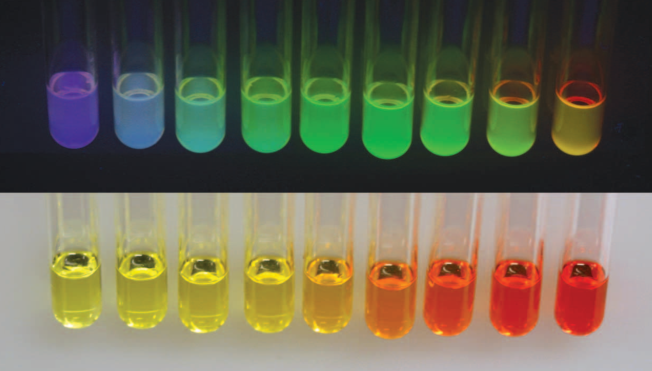
\includegraphics[width=0.8\textwidth]{./figures/colors.png}
	\caption{Various aliquots of CdSe nanocrystals, arranged from left to
	right in order of increasing size. Below: Color of CdSe quantum dots under
ambient conditions. Above: Color of CdSe quantum dots under a UV blacklight.
Reprinted from Boatman and colleagues. \cite{jce-2}}
\end{figure}

\begin{figure}[ht]%
	\centering%
	\begin{subfigure}[b]{0.5 \textwidth}%
		\centering%
		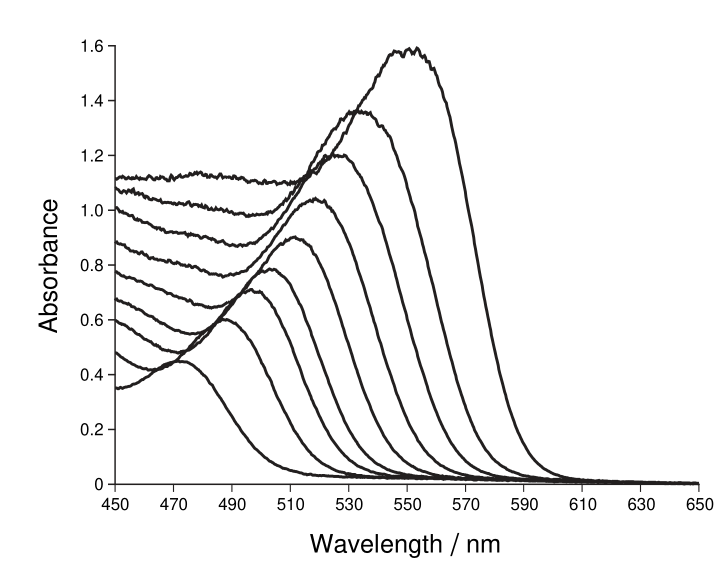
\includegraphics[width=\textwidth]{./figures/absorbance}%
		\subcaption{}%
	\end{subfigure}%
	\hfill%
	\begin{subfigure}[b]{0.5 \textwidth}%
		\centering%
		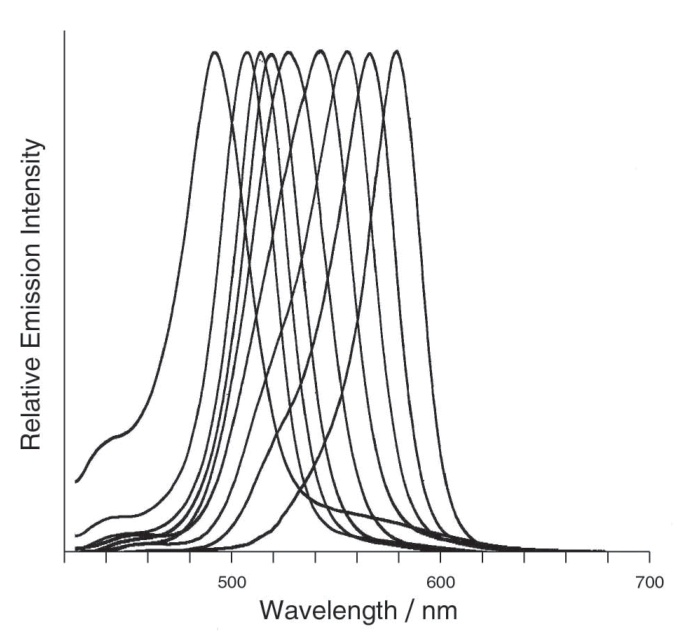
\includegraphics[width=\textwidth]{./figures/emission}%
		\subcaption{}%
	\end{subfigure}%
	\caption{Absorbance spectra (a) and fluroescent emission spectra at 400
	nm excitation (b) of CdSe nanocrystals of various sizes. Larger
	nanocrystals correspond to higher wavelength absorbance and emission. Reprinted
	from Boatman and colleagues. \cite{jce-2}}%
\end{figure}%

Rather than using yield as the basis of reaction quality, monodispersity should
be used. Monodispersity can be determined by the peak width (full-width,
half-maximum) of the absorbance and fluroescence spectral peaks, with thinner
peaks indicating a higher degree of monodispersity. Instructors may also provide
spectra of nanocrystals both before and after ripening, and ask students to
interpret differences between the spectra.

Absorbance and fluorescence spectra should reveal that larger CdSe nanocrystals
(taken from aliquots which underwent a longer reaction time) have
correspondingly redshifted absorbance and emission peaks. This is in agreement
with the theoretical Wannier-Mott exciton band gap detailed in the introduction
and summarized in Equation (2), which predicts a lower band gap for larger
nanocrystals. These spectra should resemble those presented in Figure 2, but
with less background at lower wavelengths due to the removal of impurities
during centrifugation.

\begin{figure}[H]
	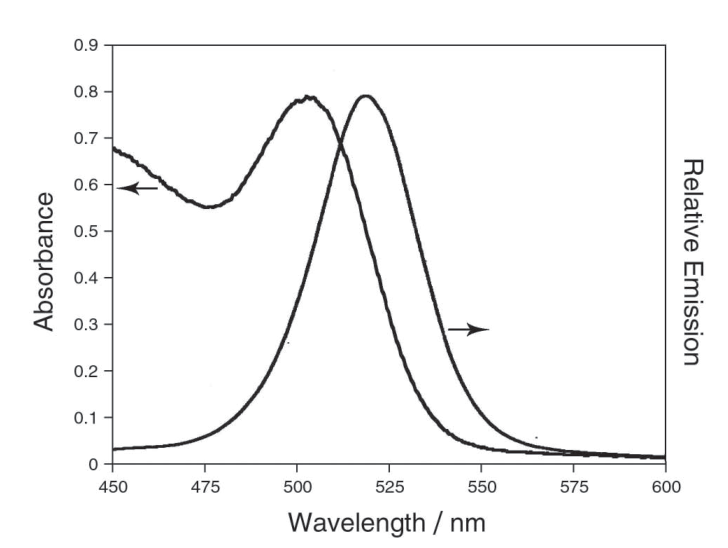
\includegraphics[width=0.8\textwidth]{./figures/stokes.png}
	\caption{Stokes shift observed for a given size CdSe quantum dot.
	Reprinted from Boatman and colleagues. \cite{jce-2}}
\end{figure}

There should be a noticable Stokes shift between the wavelengths of the
absorbance and emission peaks, coupled with a lower peak width of emission
peaks, as shown in Figure 3. Especially gifted students should be able to
explain these two phenomena in terms of non-radiative transitions and selection
rules.

\section{Conclusion}

% Conclusion (10 points). This can be just a paragraph.

\newpage

\bibliography{bib.bib}

\end{document}
